\chapter{Related Work}
\label{ch:Related-Work}

This chapter introduces and explains terms and concepts which will be used throughout the thesis. Thus, this section can be used as a reference guide to fill in any gaps and to understand the relationships between the individual concepts better.

\section{Introduction to Digital Signal Processing}
\label{sec:Intro-DSP}

This section introduces the fundamentals of \gls{DSP}, which will be used repeatedly in the following chapters, either to reason or to describe some behaviour. 
\newline
\newline
What exactly is \gls{DSP}? \gls{DSP} is to take real-world signals like voice, audio, video, temperature, pressure, or position that have been digitized and mathematically manipulate them. A \gls{DSP} is designed for performing mathematical functions such as \textit{add}, \textit{subtract}, \textit{multiply} and \textit{divide} very quickly.
\newline
\newline
Signals need to be processed so that the information that they contain can be displayed, analyzed, or converted to another type of signal that may be of use. In the real-world, analogue products detect signals such as sound, light, temperature or pressure and manipulate them. Converters such as an \gls{ADC} then take the real-world signal and turn it into the digital format of 1's and 0's. From here, the \gls{DSP} takes over by capturing the digitized information and processing it. It then feeds the digitized information back for use in the real world. It does this in one of two ways, either digitally or in an analogue format by going through a \gls{DAC}. All of this occurs at very high speeds.\footnotemark

\footnotetext{\href{https://www.analog.com/en/design-center/landing-pages/001/beginners-guide-to-dsp.html}{analog.com/en/design-center/landing-pages/001/beginners-guide-to-dsp.html}}

\subsection{Waveform}
\label{sub:Waveform}

Speech signals are sound signals, defined as pressure variations travelling through the air. These variations in pressure can be described as waves, and are often called sound waves. In the current thesis, the focus is on the analysis and processing of such waveforms in digital systems. Therefore it is always assumed that the acoustic speech signals have been captured by a microphone and converted to a digital form.
\newline
\newline
A speech signal is represented by a sequence of numbers $x_n$, which represent the relative air pressure at time-instant $n\in{\mathbb N}$. The accuracy of this representation is specified by two variables, the sampling frequency (the step in time between $n$ and $n+1$) and the accuracy and distribution of amplitudes of $x$.

\subsection{Amplitude}
\label{sub:Amplitude}

The amplitude of a periodic variable is the measure of how far, and in what direction, that variable differs from zero. Thus, signal amplitudes can be either positive or negative. The figure \ref{fig:Amplitude-Wavelenght} illustrates the amplitude with variable $y$. If the amplitude of a given signal is large, the signal is observed to be loud.
\newline
\newline
The distance from the top of one peak to the bottom of another is called \textit{peak-to-peak amplitude}. Another way to describe peak-to-peak amplitude is to say that it is the distance between the maximum positive value and the maximum negative value of a wave. In figure \ref{fig:Amplitude-Wavelenght}, the peak-to-peak amplitude of the wave would be $2y$.

\subsection{Magnitude}
\label{sub:Magnitude}

The magnitude of a periodic variable is the measure of how far, regardless of direction, its quantity differs from zero. So magnitudes are always positive values. Occasionally, in the literature of digital signal processing, the term magnitude is referred to as the absolute value. In figure \ref{fig:Amplitude-Wavelenght}, the magnitude of the wave would be $|y|$.

\subsection{Wavelength}
\label{sub:Wavelength}

The wavelength is the length of a single cycle of a wave, as measured by the distance between one peak of a wave and the next. In figure \ref{fig:Amplitude-Wavelenght} the wavelength is designated as the variable $\lambda$.

\subsection{Frequency}
\label{sub:Frequency}

Frequency is the number of occurrences of a repeating event per unit of time. It depends on the wavelength of an audio signal $\lambda$. The frequency is given by the equation \ref{eq:Frequency}. If the signal at a given time has a high frequency, it is observed to have a higher pitch.

\myequations{Calculate frequency from wavelength}
\begin{equation}
    \centering
    f = \frac{1}{\lambda}
    \label{eq:Frequency}
\end{equation}

\begin{figure}[htbp]
	\centering
	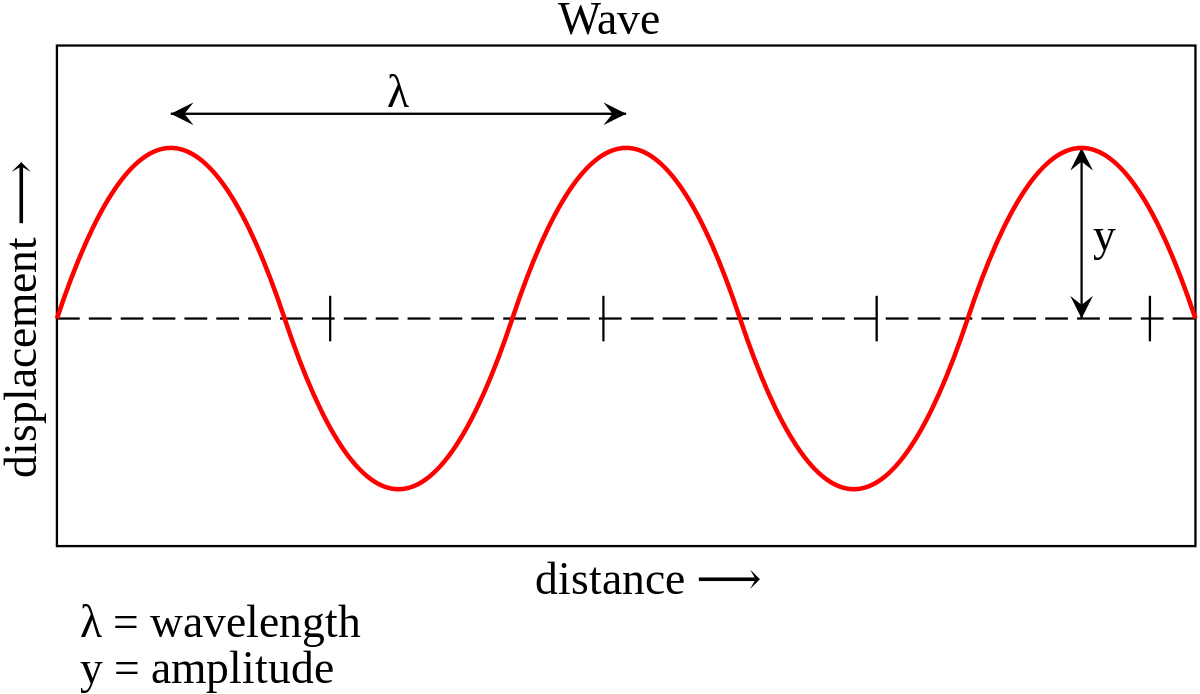
\includegraphics[scale=0.25]{baa-documentation/img/Amplitude.png}
	\caption[Amplitude and wavelength illustrated]{Amplitude and wavelength \footnotemark}
	\label{fig:Amplitude-Wavelenght}
\end{figure}
\footnotetext{\href{https://en.wikiversity.org/wiki/Amplitude}{\nolinkurl{en.wikiversity.org/wiki/Amplitude}}}

\subsection{Sampling}
\label{sub:Sampling}

Sampling is the first step to convert an analogue signal to a digital one. Firstly the signal has to be sampled using a device called an \gls{ADC}. The \gls{ADC} will measure the signal at rapid intervals, and these measurements are called samples. It will output a digital signal proportional to the amplitude of the analogue signal at that same instant. The rate at which the \gls{ADC} will measure the analogue signal is called the \textbf{sample rate}.

\subsection{Aliasing}
\label{sub:Aliasing}

Aliasing is a special effect that can happen when the speed of samples taken from the analogue signal is to low compared to the actual analogue signal, otherwise known as frequency. Aliasing is due to the fact that the actual signal is changing so rapidly between sampling instants, that this rapid movement is not visible in the sampled signal. The sampled signal appears to be a lower frequency signal compared to the actual signal.

\subsection{Quantization}
\label{sub:Quantization}

Quantization is the process of mapping input values from a large continuous set (analogue signal) to output values in a smaller collection (digital signal), with a finite number of elements. Not all input values can be represented in the finite set, so the values have to be mapped to an existing number in it, called quantized value. This is usually done by rounding or truncation. The difference between an input value and its quantized value is referred to as quantization error.  If more bits are available in the digital signal, then the quantization error gets smaller and also the digital signal has a higher quality. This number of bits in a signal is called the \textbf{bit depth}. A device or algorithmic function that performs quantization is called a quantizer. An \gls{ADC} is an example of a quantizer. 

\subsection{Sampling Frequency and Resolution}
\label{sub:Sampling-Frequency-Resolution}

The sampling frequency or sampling rate, given in \gls{Hz}, of an audio signal, determines the resolution of the audio sample. The sampling frequency states how many samples (amplitudes \ref{sub:Amplitude}) were captured for each second of the signal. Each one of these samples also has a resolution, given in bits, which determines how detailed audio waveforms are. This resolution is also referred to as bit depth. The higher the sampling rate, the higher the resolution of the signal. When recording music or many types of acoustic events, audio waveforms are typically sampled at 44.1 \gls{kHz} (CD), 48 \gls{kHz}, 88.2 \gls{kHz}, or 96 \gls{kHz}. Sampling rates higher than about 50 \gls{kHz} to 60 \gls{kHz} cannot supply more usable information for human listeners. Early professional audio equipment manufacturers chose sampling rates in the region of 40 to 50 \gls{kHz} for this reason.

\subsection{Nyquist–Shannon sampling theorem}
\label{sub:Nyquist–Shannon}

This theorem was introduced to prevent the \nameref{sub:Aliasing} phenomenon and give some rule or convention to sampling. The Nyquist-Shannon sampling theorem implies, to sample more than twice as fast as the signal to convert.
\newline
\newline
Whenever a sampled signal is given, there is no certainty that the signal represents the analogue one. However, if the signal was sampled at more than twice the frequency of the signal, then the sampled signal will accurately represent the same frequency as the actual signal ere sampling. The critical frequency which the signal must not ever exceed, which is precisely one half of the sampling frequency, is called the Nyquist frequency.

\subsection{Noise}
\label{sub:Noise}

Noise is any unwanted signal distorting the original signal. Given a speech signal with amplitude $s(n)$, where $n$ is the sample index, noise is any other signal, $w(n)$ which interferes with the speech. The noisy speech signal $u(n)$ is defined with equation \ref{eq:Noise-Added}.

\myequations{Noise added to a signal}
\begin{equation}
    \centering
    u(n) = s(n) + w(n)
    \label{eq:Noise-Added}
\end{equation}

\subsection{Time domain}
\label{sub:Time-Domain}

The time-domain refers to the analysis of mathematical functions of signals with respect to time. A time-domain graph shows how a signal changes with time. 
\newline
\newline
A wave plot is a visual representation of this domain. The y-axis of such visualisation represents the \nameref{sub:Amplitude} (loudness) of the sound wave, whereas the x-axis represents the time. If the amplitude is equal to zero, it represents silence. Such a representation is shown in figure \ref{fig:Waveplot-Time-Domain}.
\begin{figure}[htbp]
	\centering
	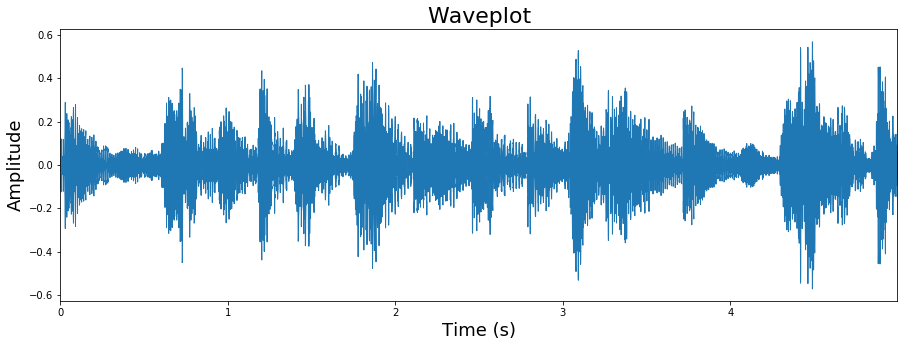
\includegraphics[scale=0.45]{baa-documentation/img/Waveplot_Visualisation.png}
	\caption[Time-domain illustrated in wave plot]{Time-domain illustrated in wave plot}
	\label{fig:Waveplot-Time-Domain}
\end{figure}

\subsection{Frequency domain}
\label{sub:Frequency-Domain}

The frequency-domain refers to the analysis of mathematical functions or signals with respect to frequency. A frequency-domain graph shows how much of the signal lies within each given frequency band over a range of frequencies. 
\newline
\newline
A given function or signal can be converted between the time and frequency domains with a pair of mathematical operators. The most used operation is the Fourier Transformation, which will be explained in further detail in section \ref{sub:Fourier-Transform}.

\subsection{Fourier Transform}
\label{sub:Fourier-Transform}

\gls{FT} is a mathematical concept that can convert a continuous signal from \fullref{sub:Time-Domain} to \fullref{sub:Frequency-Domain}. It decomposes a complex periodic signal into its constituent sine waves oscillating at different frequencies, along with the magnitude of each wave. The magnitude of each frequency shows how much a certain wave contributes to the overall signal.

\subsubsection{Fast Fourier Transform}
\label{subsub:Fast-Fourier-Transform}

\gls{FFT} is a mathematical algorithm that calculates \gls{DFT} of a given sequence, with the equation \ref{eq:DFT}. The only difference between \gls{FT} and \gls{FFT} is, that \gls{FT} considers a continuous signal while \gls{FFT} takes a discrete signal as input. \gls{DFT} converts a sequence, a discrete signal, into its frequency constituents just like \gls{FT} does for a continuous signal. It is important to note that due to that transformation, the time information of the audio signal will be lost.

\myequations{Discrete Fourier Transform}
\begin{equation}
    \centering
    X_k = \sum_{n=0}^{N-1} \ x_n \cdot e^{-\frac{i2\pi}{N}kn}
    \label{eq:DFT}
\end{equation}

\subsubsection{Short Time Fourier Transform}
\label{subsub:Short-Time-Fourier-Transform}

\gls{STFT} is a mathematical algorithm which addresses the issue, that in the \nameref{sub:Frequency-Domain} no time information exists. The \gls{STFT} calculates several \gls{FFT} at different time intervals and combines them to get information about the signal varying over time.

\subsection{Spectrogram}
\label{sub:Spectrogram}

A spectrogram is a visual representation of the \nameref{subsub:Short-Time-Fourier-Transform}. More precisely it represents the spectrum of frequencies of a signal as it varies with time. The x-axis represents the time, the y-axis represents the frequencies, and the colours represent the magnitude of the observed frequency at a particular time. Bright colours represent powerful frequencies. Thus every spectrogram represents three domains: time, frequency and magnitude.
\newline
\newline
To create a spectrogram, the audio signal is broken down into smaller frames (windows), and for each one, the \gls{DFT} or \gls{FFT} will be calculated. The resulting frequencies of each window will represent the time. It is important to note that the windows should overlap each other, not to lose any frequency. Typical window sizes are 20 to 30ms, but this size highly depends on the task to solve. The figure \ref{fig:Spectrogram} show an example of such a spectrogram.
\begin{figure}[htbp]
	\centering
	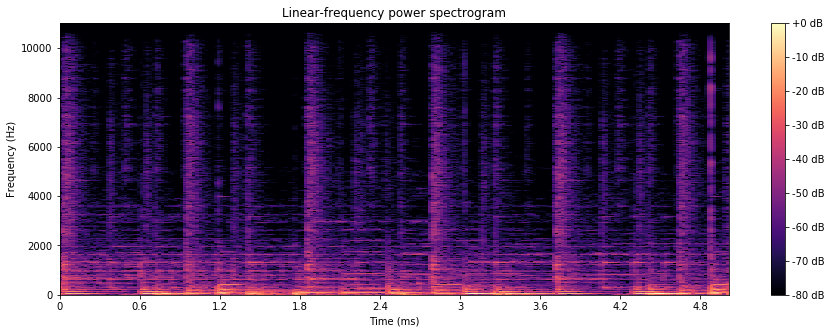
\includegraphics[scale=0.5]{baa-documentation/img/Spectrogram_Visualisation.png}
	\caption[Example of a spectrogram]{Example of a spectrogram}
	\label{fig:Spectrogram}
\end{figure}

\subsection{Mel Spectogram}
\label{sub:Mel-Spectogram}

\gls{MFCC} are a feature widely used in automatic speech and speaker recognition, mainly because they focus on the audio signal and discard all other information such as background noise, emotion and many more. They were introduced by Davis and Mermelstein in the 1980s, and have been state-of-the-art ever since.
\newline
\newline
The process of creating these \gls{MFCC} are quite complex and follow five steps. Thus to the explanation of every step, there is also a short example on how to perform the step in depth. For illustration, a speech signal with a sample rate of 16kHz is assumed. The whole process is illustrated in figure \ref{fig:MFCC-Overview}.

% TODO - create own diagram
\begin{figure}[htbp]
	\centering
	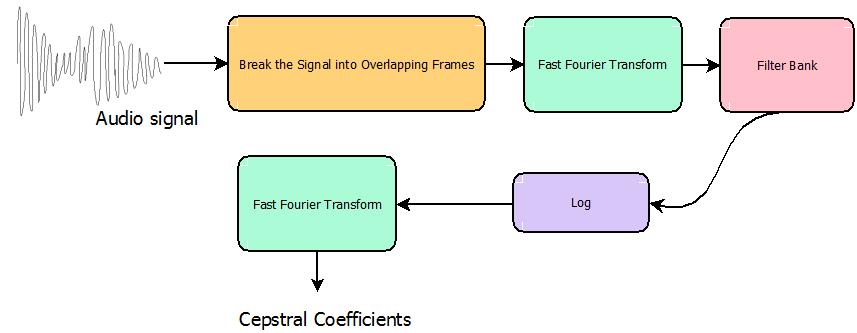
\includegraphics[scale=0.8]{baa-documentation/img/MFCC_Overview.jpeg}
	\caption[Steps to calculate MFCC]{Steps to calculate MFCC \footnotemark}
	\label{fig:MFCC-Overview}
\end{figure}
\footnotetext{\href{https://mitll.github.io/pyslgr/MFCC_Features.html}{\nolinkurl{mitll.github.io/pyslgr/MFCC_Features.html}}}

\subsubsection{Frame the signal into short frames}
An audio signal is continuously changing, so to simplify it is assumed, that on short time scales the audio signal does not change much, i.e. statistically stationary. Due to that, the signal is framed into 20-40ms frames. If the frames are much shorter, there are not enough samples to get a reliable spectral estimate. If the frame length is too high, the signal changes to much throughout the frame.
\newline 
\newline
Firstly the signal has to be split into 20-40ms frames (25ms is the standard). The frame length for a 16kHz signal is calculated with the equation in \ref{eq:MFCC-Frame-Length}. 
\myequations{Calculate frame length from signal}
\begin{equation}
    \centering
    \frac{25ms}{1000} \ 16000Hz = 400 \ \text{samples}
    \label{eq:MFCC-Frame-Length}
\end{equation}
Frame step is normally 10ms, which allows some overlap to the frames, and is calculated the same as the frame length.
\myequations{Calculate frame step from signal}
\begin{equation}
    \centering
    \frac{10ms}{1000} \ 16000Hz = 160 \ \text{samples}
    \label{eq:MFCC-Frame-Step}
\end{equation}
This means that the first 400 samples start at 0, the next 400 frames start at sample 160, until the end of the speech signal is reached. If the speech signal does not divide into an even number of frames, it is padded with zeros until it does. The next steps in the example are applied to every single frame, one set of 12 \gls{MFCC} is extracted for each frame.

\subsubsection{Calculate the periodogram estimate of the power spectrum for each frame}
The next step is to calculate the power spectrum of each frame. This is motivated by the human cochlea, an organ in the ear, which vibrates at different spots depending on the frequency of the incoming sounds. Depending on which location in the cochlea that vibrates, different nerves fire, informing the brain that specific frequencies are present. The periodogram estimate performs a similar job which is, identifying which frequencies are present in the frame.
\newline
\newline
To calculate the power spectrum for each frame, the \gls{DFT} has to be calculated with the equation \ref{eq:MFCC-DFT-Frame}. Then the Periodogram-based power spectral estimate for the speech frame $s_i(n)$ can be calculated with the formula \ref{eq:MFCC-Periodogram-Frame}. Usually a 512 point \gls{FFT} is being performed and only the first 257 coefficients are kept.
% TODO - check equation
\myequations{Calculate Discrete Fourier Transform of each frame}
\begin{equation}
    \centering
    S_i(k) = \sum_{n=1}^{N} s_i(n) h(n) e^{- \frac{i2\pi}{N} kn} \qquad 1 \leq k \leq K
    \label{eq:MFCC-DFT-Frame}
\end{equation}
\myequations{Calculate Periodogram-based power spectral estimate of each frame}
\begin{equation}
    \centering
    P_i(k) = \frac{1}{N}|S_i(k)|^2
    \label{eq:MFCC-Periodogram-Frame}
\end{equation}
where:
\begin{conditions*}
 s_i(n) &  time domain signal frame, where $n$ denotes the frame length (in the current example from 1-400) and $i$ ranges over the number of frames \\   
 S_i(k) &  complex \gls{DFT}, where $i$ denotes the frame number corresponding to the time-domain frame \\
 h(n)   &  analysis window, with the size $N$ (e.g. hamming window) \\
 K      &  length of the \gls{DFT} \\
 P_i(k) &  power spectrum of frame $i$
\end{conditions*}

\subsubsection{Apply the mel filterbank to the power spectra}
The periodogram spectral estimate still contains much information not required for \gls{ASR}. In the human body, the cochlea can not discern the difference between two closely spaced frequencies. This effect becomes more pronounced as the frequencies increase. For this reason, clumps of periodogram bins and sums are taken and summed up, to get an idea of how much energy exists in various frequency regions.
\newline
\newline
The Mel filterbank performs this step. The first filter of the filterbank is very narrow and indicates how much energy exists near 0 Hertz. As the frequencies get higher, the filters get wider as the variations become less relevant. The interest is only focused on how much energy occurs at each spot. The Mel scale gives the spacing and the wideness of the filterbanks. It relates perceived frequency, or pitch, of a pure tone to its actual measured frequency, it transforms the features to match more closely what humans hear. The equation \ref{eq:MFCC-Mel} converts a frequency ($f$) to the Mel scale ($m$) and equation \ref{eq:MFCC-Mel-Inv} transforms the Mels ($m$) back to a frequency ($f$).\footnote{\fullcite{anne_acoustic_2015}}
\myequations{Calculate Mel scale from frequency}
\begin{equation}
    \centering
    m = 2595 \ log_{10}(1 + \frac{f}{700Hz}) = 1127 \ log_e(1 + \frac{f}{700Hz})
    \label{eq:MFCC-Mel}
\end{equation}
\myequations{Calculate frequency from Mel scale}
\begin{equation}
    \centering
    f = 700 \ (10^{m/2595-1}) = 700 \ (e^{m/1127-1})
    \label{eq:MFCC-Mel-Inv}
\end{equation}
The Mel-spaced filterbank has to be computed to apply the filterbank to the power spectra. The filterbank is a set of 20-40 (26 is the standard) triangular filters that then are applied to the periodogram from before. The filterbank has the dimension of 26 vectors with the length 257, because in the step before we calculated the \gls{FFT} and only kept 257 coefficients. Each vector has mostly zeros in it but is non-zero for a specific section of the spectrum. Each filterbank has to be multiplied by the power spectrum. After that, the coefficients are added up to get the filterbank energies. In the end, there are 26 coefficients left, which indicates how much energy was in each filterbank. An example of a Mel-spaced filterbank is illustrated in \ref{fig:MFCC-Mel-Filterbank}.
\begin{figure}[htbp]
	\centering
	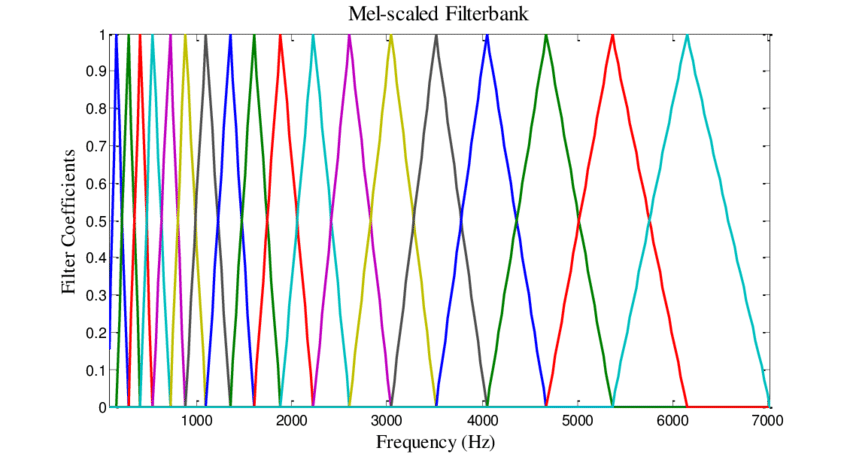
\includegraphics[scale=0.4]{baa-documentation/img/Mel-filter-banks-basis-functions-using-20-Mel-filters-in-the-filter-bank.png}
	\caption[Mel-spaced filterbank with 20 filters]{Mel-spaced filterbank with 20 filters \footnotemark}
	\label{fig:MFCC-Mel-Filterbank}
\end{figure}
\footnotetext{\fullcite{mohd_ali_analysis_2013}}

\subsubsection{Apply the logarithm to all filterbank energies}
After we calculated the filterbank energies, the logarithm is applied to each one of them. This operation is also inspired by human hearing because humans do not hear loudness on a linear scale. Generally to double the perceived volume of a sound eight times as much energy has to be put in. Thus if the sound signal is loud in the beginning, significant variations in energy may not sound that different.
\newline
\newline
In our example, we now have 26 energy coefficients which will be logarithmized which leaves 26 log filterbank energies.

\subsubsection{Apply the \gls{DCT} to the log filterbank energies}
The final step is to compute the \gls{DCT} of the log filterbank energies. Mainly because the filterbanks are all overlapping and are correlated with each other. The \gls{DCT} decorrelates the energies, but only the lower 12-13 of the 26 \gls{DCT} coefficients are kept. This is because the higher \gls{DCT} coefficients represent fast changes in the filterbank energies, and these fast changes can degrade the \gls{ASR} performance.
\newline
\newline
In the example the \gls{DCT} of the 26 log filterbank energies has to be computed, which gives 26 cepstral coefficients. This whole process has to be calculated for each frame in the signal.

\subsubsection{Visualize the cepstral coefficients}
Once all the cepstral coefficients are computed, they can be visualized with respect to time. Which then can be used for further processing in \gls{ASR}. Such a visualisation is illustrated in figure \ref{fig:MFCC-Visualisation}, where the x-axis represents the time and the y-axis represents the cepstral coefficient dimension (e.g. the lower 12-13) and the color shows the value of each coefficient.
\begin{figure}[htbp]
	\centering
	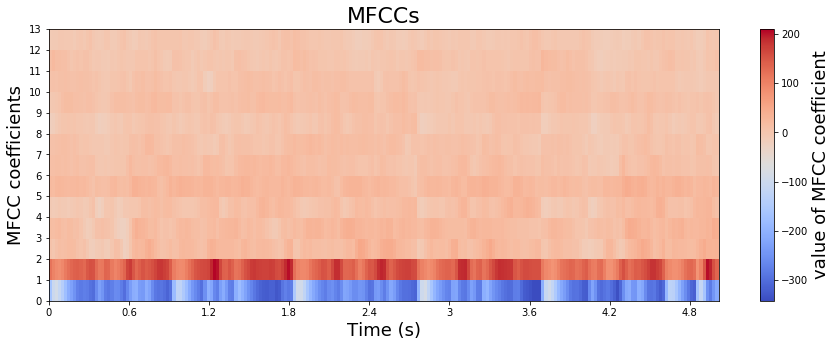
\includegraphics[scale=0.5]{baa-documentation/img/MFCC_Visualisation.png}
	\caption[Visualisation of a MFCC]{Visualisation of a MFCC}
	\label{fig:MFCC-Visualisation}
\end{figure}

\subsection{$\mu$-law Transformation}
\label{sub:Mu-Law-Transformation}

\subsection{LibROSA}
\label{sub:Librosa}

LibROSA is a python package for music and audio analysis. It provides the building blocks necessary to create music information retrieval systems.\footnote{\url{https://librosa.github.io/librosa/}}

\section{Introduction to Neural Nets}
\label{sec:Intro-NN}

In this section, technical concepts are explained in more detail, which was used in the thesis. These concepts are mostly very complex and are, therefore only touched upon so that the further conclusions of this work can be understood comprehensibly.

\subsection{Neural Nets}
\label{sub:Neural-Nets}

\subsection{Convolutional Neural Nets}
\label{sub:Convolutional-Neural-Nets}

\subsection{Gated Linear Unit}
\label{sub:Gated-Linear-Unit}

\subsection{Tensorflow}
\label{sub:Tensorflow}

TensorFlow is an end-to-end open source platform for machine learning. It has a comprehensive, flexible ecosystem of tools, libraries and community resources that lets researchers push the state-of-the-art in \gls{ML} and developers easily build and deploy \gls{ML} powered applications. \footnote{\url{https://www.tensorflow.org/}}

\section{State of the art}
\label{sec:State-of-art}

\subsection{Word2Vec}
\label{sub:word2wec}

\subsection{Triplet Loss}
\label{sub:Triplet-Loss}

\section{Status in relation to project}
\label{sec:Status-Relation-Project}
